\chapter{Background}

\section{Optimisation}

Optimisation is the process to finding the optimal decision with respect to constraints given a set of possible decisions. The optimal decision is measured by a cost function, that typically determines a numerical value representing how good a decision is. The problem is to either find the optimal decision, either as a minima or maxima using systematic methods. Applications of optimisation occur in many practical situations such as in engineering, manufacturing, science. In engineering applications, accurate modelling of a problem may require discrete decisions and non-linear relationships, resulting in difficulty in finding arbitrary optimal decisions. The wide range of applications of optimisation result in  many fields of optimisation, where in this project we look at MILP.
\begin{center}
	\begin{tikzpicture}
		\node[file](problem) at (0, 2){Problem};
		\node[file](model) at (0, 0){Model};
		\node[file](solution) at (4, 2){Solution};
		\node[file](optimum) at (4, 0){Optimum};
		\draw[arrow](problem) -- node [above] {solve} (solution);
		\draw[arrow](problem) -- node [left, inner sep=10pt] {abstact} (model);
		\draw[arrow](model) -- node [below] {optimise} (optimum);
		\draw[arrow](optimum) -- node [right, inner sep=10pt] {intepret} (solution);
	\end{tikzpicture}
\end{center}
Real-life problems need to be modelled to be optimised. Problems are formulated using constraints and a cost function. Consider the following linear programming example. A person want to sell some drinks. Each unit of hot chocolate requires 1 litre of milk and 3 bars of chocolate. Each unit of milkshake requires 1 litre of milk and 2 bars of chocolate. The person only has 5 units of milk and 12 bars of chocolate. The person sells a unit of hot chocolate for £6 and a unit of milkshake for £5. What is the best strategy for maximising profit given that all units produced are sold? The problem is abstracted as follows. Let $x$ and $y$ be the number of hot chocolates and milkshakes produced.
\begin{align*}
	\max_{x,y}\ &6x+5y&\text{subject to:}\\
	&x+y\leq 5&\text{milk resource constraint}\\
	&3x+2y\leq 12&\text{chocolate resource constraint}\\
	&x,y\geq 0&\text{non-negative constraints}\\
	&x,y\in\mathbb{N}&\text{whole units only}\\
\end{align*}
The problem is sufficiently small to be solved by inspection, but may also be solved using graphical methods or a simplex algorithm. The optimum is $x^*=2$ and $y^*=3$, which is interpreted as that the best strategy is producing 2 units of hot chocolate and 3 units of milkshake.
\linespace
In non-linear optimisation problems, finding global optimums in not trivial. For gradient-based and local-search algorithms, estimated solutions can return local optimums. This is typically not favoured however for large problems, finding global optimums have non-polynomial complexity. In context of the project, it would not be feasible to compute an explanation in polynomial time.

\subsection{Makeshift Scheduling}

The simplistic definition of makeshift scheduling gives a good foundation for experimenting with argumentation. Makeshift schedules are defined by a $m\in\mathbb{N}$ independent machines and $n\in\mathbb{N}$ independent jobs.\cite{sa} Let $\mathcal{M}=\{1,...,m\}$ be the set of machines and $\mathcal{J}=\{1,...,n\}$ be the set of jobs. Each job $i\in\mathcal{J}$, has an associated processing time $p_i\in\mathbb{R}_{\geq 0}$. All processing times are collectively denoted by a vector $\mathbf{p}$. A machine can only execute at most one job at any time. For a feasible schedule, each job is assigned to a machine non-preemptively. For some $i\in\mathcal{M}$, let $C_i$ be the completion time of the $i^\text{th}$ machine. Let $C_{\max}$ be the total completion time. Let $\mathbf{x}\in\{0,1\}^{m\times n}$ be the assignment matrix that allocates jobs to machines. Formally, makeshift schedules are modelled as an optimisation problem:
\begin{align*}
	\min_{C_{\max},\mathbf{C},\mathbf{x}}&C_{\max}&\text{ subject to:}\\
	\forall i\in\mathcal{M}.\ &C_{\max}\geq C_i\\
	\forall i\in\mathcal{M}.\ &C_i=\sum_{j\in\mathcal{J}}x_{i,j}\cdot p_j\\
	\forall j\in\mathcal{J}.\ &\sum_{j\in\mathcal{J}}x_{i,j}=1\\
	\forall i\in\mathcal{M},\ \forall j\in\mathcal{J}.\ &x_{i,j}\in\{0,1\}
\end{align*}

\begin{definition}
	A schedule $S$ is defined by its assignment matrix $\mathbf{x}$ such that $S=\mathbf{x}$.
\end{definition}

\begin{definition}
	A schedule $S$ is optimal iff $S$ achieves the minimal total completion time.
\end{definition}


\begin{definition}
	A machine $i\in\mathcal{M}$ is critical iff $C_i=C_{max}$.
\end{definition}

\begin{definition}
	A job $j\in\mathcal{J}$ is critical iff $j$ is allocated to a critical machine $i\in\mathcal{M}$ such that $x_{i,j}=1$.
\end{definition}

\begin{definition}
	A schedule satisfies the single exchange property (SEP) iff for any critical machine and any machine $i,i'\in\mathcal{M}$ and for all critical jobs $j\in\mathcal{J}$, $C_i-C_{i'}\leq p_j$
\end{definition}

\begin{definition}
	A schedule satisfies the pairwise exchange property (PEP) iff for any critical job and any job $j,j'\in\mathcal{J}$, if $p_j>p_{j'}$, then $C_i+p_{j'}\leq C_{i'}+p_j$.
\end{definition}

\begin{definition}
	A schedule $S$ is efficient iff $S$ satisfies SEP and PEP.
\end{definition}

\begin{theorem}
	Schedule efficiency is a necessary condition for optimality.
\end{theorem}

\subsection{User Fixed Decisions}

To accommodate practical applications of makeshift schedules, user positive and negative fixed decisions are introduced as an extension. In a hospital setting, positive fixed decisions capture patients exclusively allocated to a nurse while negative fixed decisions capture unavailable or incompatible nurses and patients. Let $D^-,D^+\subseteq\mathcal{M}\times\mathcal{J}$ be the negative and positive fixed decisions respectively. Let $D$ be the fixed decisions such that $D=(D^-,D^+)$.

\begin{definition}
	A schedule $S$ satisfies $D$ iff $\forall(i,j)\in D^-.\ x_{i,j}=0$ and $\forall (i,j)\in D^+.\ x_{i,j}=1$.
\end{definition}

\begin{definition}
	A fixed decision $D$ is satisfiable iff there exists a schedule $S$ such that $S$ satisfies $D$. 
\end{definition}

\begin{theorem}
	A fixed decision $D$ is unsatisfiable iff if the following necessary and sufficient conditions hold:
	\begin{itemize}
		\item$D^+$ and $D^-$ are disjoint.
		\item$\forall(i,j),(i',j')\in D^+.\ i=i'\lor j\neq j'$
		\item$\forall j\in\mathcal{J}.\ \exists i\in\mathcal{M}.\ (i,j)\not\in D^-$
	\end{itemize}
\end{theorem}

Makeshift schedules are often represented using cascade charts.

\begin{center}
	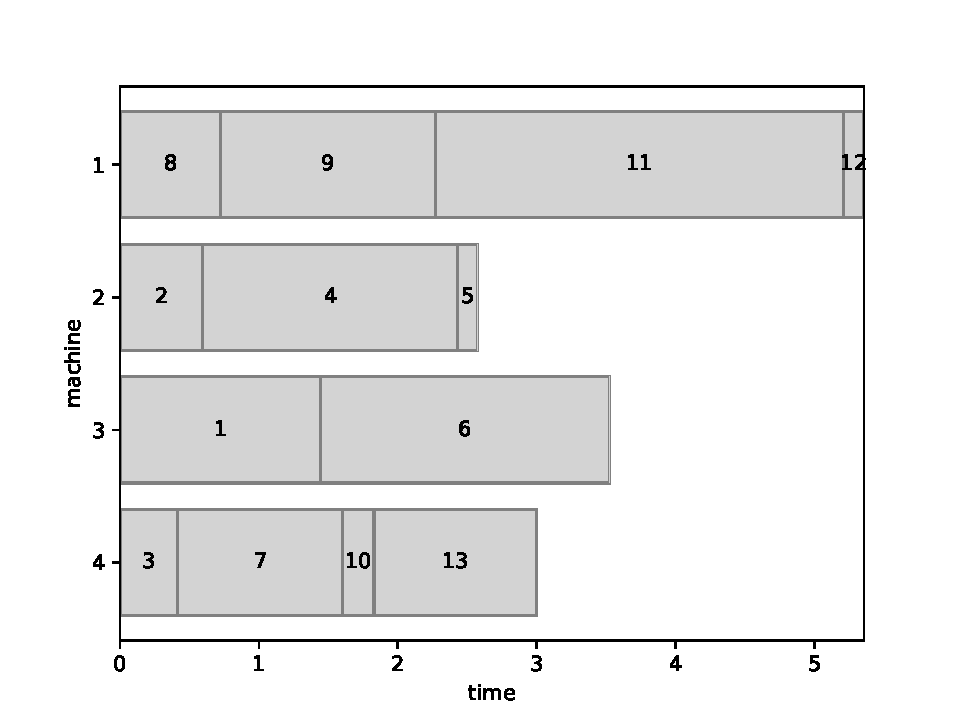
\includegraphics[width=.6\linewidth]{figures/makeshift1.pdf}
\end{center}

\begin{center}
	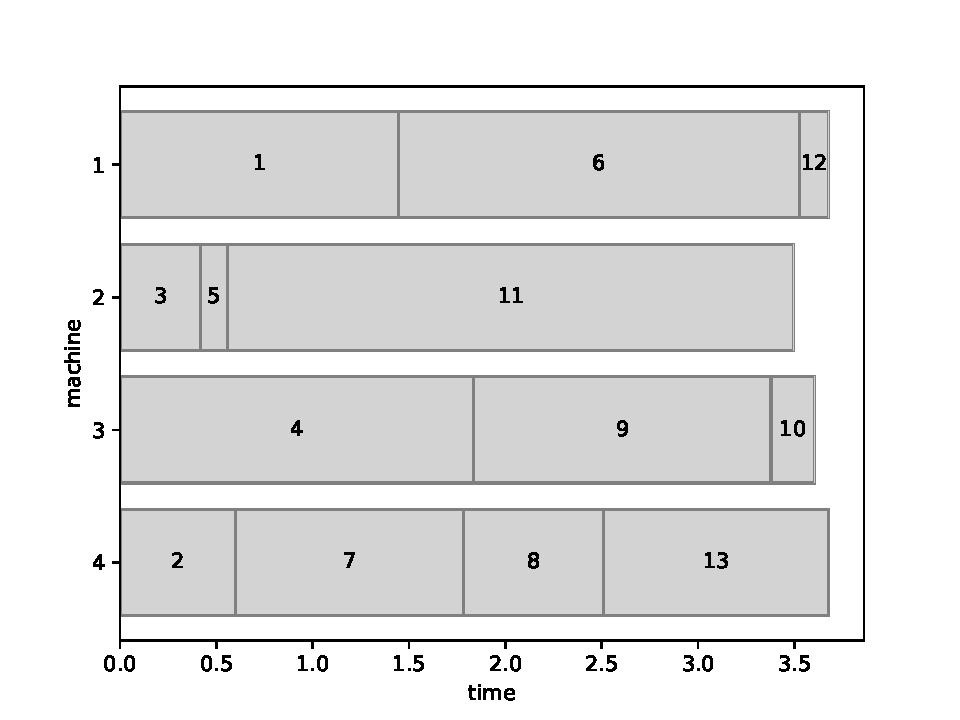
\includegraphics[width=.6\linewidth]{figures/makeshift2.pdf}	
\end{center}

\subsection{Interval Scheduling}

...

\section{Argumentation}

Argumentation is a method to understand and evaluate reasons for and against potential conclusions. Argumentation is useful in resolving conflicts, clarifying incomplete information and most importantly, with respect to this project, explanations. The precise definition of an argument varies on the literature, however it is commonly agreed that arguments can attack or support other arguments. For an argument $\alpha$ to attack an argument $\beta$, $\alpha$ may critically challenge $\beta$ such that acceptability of $\beta$ is doubted.\cite{at} This may be to question one of $\beta$'s premises, by proposing a counter-example. For example, consider an scenario whether to sleep. Let $\alpha$ be ``I want to sleep", $\beta$ be ``I have work to do" and $\gamma$ be ``I can work tomorrow". Using human intuition, we can derive that $\gamma$ attacks $\beta$ and $\beta$ attacks $\alpha$. This is represented graphically below.

\begin{center}
	\begin{tikzpicture}
		\node[node](gamma) at (0, 0){$\gamma$};
		\node[node](beta) at (2, 0){$\beta$};
		\node[node](alpha) at (4, 0){$\alpha$};
		\draw[arrow](gamma) -- (beta);
		\draw[arrow](beta) -- (alpha);
	\end{tikzpicture}
\end{center}

If we conclude $\alpha$ to be acceptable, then we must not accept $\beta$. Accepting two arguments with conflicts can be interpreted as a contradiction or hypocritical. Hence, argumentation theory have measures of acceptable extensions, to decide whether some set of arguments are acceptable in some notion, with respect to different intuitions. This motivates to use abstract argumentation frameworks.\linespace
Note that this example uses implicit background knowledge, also known as enthymemes. In this scenario, one cannot sleep and work at the same time. To our advantage, argumentation is applied to well-defined scheduling problems, so enthymemes are inapplicable in this project.

\subsection{Abstract Argumentation Frameworks}

An abstract argumentation framework (AAF) models the relation of attacks between arguments.\cite{aa} Formally, an AAF is a directed graph $(Args,\rightsquigarrow)$ where $Args$ is the set of arguments and $\rightsquigarrow$ is a binary relation over $Args$. For $a,b\in Args$, $a$ attacks $b$ iff $a\rightsquigarrow b$. Attacks are extended over sets of arguments, where $A\subseteq Args\rightsquigarrow b\in Args$ iff $\exists a\in A.\ a\rightsquigarrow b$. An extension $E$ is a subset of $Args$.

\begin{definition}
	An extension $E$ is conflict-free iff $\forall a,b\in E.\ a\not\rightsquigarrow\ b$.
\end{definition}

\begin{definition}
	An extension $E$ is stable iff $E$ is conflict-free and
	
	$\forall a\in Args\backslash E.\ E\rightsquigarrow a$
\end{definition}

\begin{center}
	\begin{tikzpicture}
	\node[node](gamma) at (0, 0){$\gamma$};
	\node[node](beta) at (2, 0){$\beta$};
	\node[node](alpha) at (4, 0){$\alpha$};
	\node[node](delta) at (2, 2){$\delta$};
	\node[node](epsilon) at (0, 2){$\varepsilon$};
	\draw[arrow](beta) -- (alpha);
	\draw[arrow](beta) -- (gamma);
	\draw[arrow](beta) -- (delta);
	\draw[arrow](delta) -- (beta);
	\draw[arrow](delta) to [loop](delta);
	\draw[arrow](epsilon) -- (delta);
	\end{tikzpicture}
\end{center}

Consider the following example where $Args=\{\alpha,\beta,\gamma,\delta,\varepsilon\}$ and $	\rightsquigarrow=\{
\pair{\beta}{\alpha},\\
\pair{\beta}{\gamma},
\pair{\beta}{\delta},
\pair{\delta}{\beta},
\pair{\delta}{\delta},
\pair{\varepsilon}{\delta}
\}$ as illustrated above. Then the following statements hold:
\begin{itemize}
	\item $\varepsilon\rightsquigarrow\delta$.
	\item $\{\delta,\varepsilon\}\rightsquigarrow\beta$.
	\item $\{\alpha,\gamma\}$ is conflict-free but not stable.
	\item $\{\delta\}$ is not conflict-free and not stable.
	\item $\{\beta,\varepsilon\}$ is conflict-free and stable.
\end{itemize}

\section{Explanations}



\subsection{Notes}
\begin{enumerate}
	\item Conflicting negative and positive fixed decisions and explanation for their resolution
	\item Command line interface and improved graphical user interface with random, schedule display
	\item efficiency respects user fixed decisions
	\item explanations are sorted by reducible longest completion time. as m and n grows, the explanations grow. feasibility: $O(mn)$, efficiency: $O(mn^2)$, fixed decisions $O(mn)$
	\item Malle [112] explanations: find meanings, manage social interaction; learning
	\item why are explainations counterarguments: causes
	\item A tool explaining the concept of scheduling is superfluous while a tool explaining solutions concisely using mathematically-oriented may be discarded by inaccessible language. A challenge will be to strike a balance of possible explanations by targetting potential users.
\end{enumerate}

%https://ac.els-cdn.com/S0307904X12001837/1-s2.0-S0307904X12001837-main.pdf?_tid=8917b7ba-3293-40d2-a4d9-7d67b40ae499&acdnat=1546712183_67c96afaaedc7cd95cbff3dd83844cb6
